 \hoffset1cm % przesunięcie poziome (przykładowo) o 1cm przeznaczone na oprawę
 \documentclass[12pt]{report}
\usepackage[T1]{fontenc}
\usepackage[utf8]{inputenc}
\usepackage{graphicx}
\usepackage{amsmath,amssymb,amsfonts}
%\usepackage{txfonts}
\usepackage{polski}
 
 \usepackage{amsmath}
 \usepackage{amssymb}
 \usepackage{indentfirst}
 \usepackage{listings}
 \usepackage{}
% \usepackage{natbib}
 \usepackage[backend=biber, bibencoding=utf8, style=ieee, url=false, isbn=false, doi=false]{biblatex}
%  \bibliographystyle{acm}
 \addbibresource{library.bib}
 \DeclareUnicodeCharacter{229}{ę}
 \DeclareUnicodeCharacter{327}{}
 
 \pagestyle{headings}
 
\renewcommand{\chaptername}{Rozdział}
\renewcommand{\contentsname}{Spis treści}
\renewcommand{\figurename}{Rys.}
\renewcommand{\tablename}{Tab.}
\renewcommand{\listfigurename}{Spis rysunków}
\renewcommand{\listtablename}{Spis tabel}
\renewcommand{\bibname}{Bibliografia}

 \begin{document}

 \begin{titlepage}
 \center{\large\scshape Politechnika Krakowska \\
         \normalsize im. Tadeusza Kościuszki}
 \center{\scshape Wydział Inżynierii Elektrycznej i Komputerowej\\
         Kierunek Informatyka}
 \vspace{0.1\textheight}
 \center{\scshape Michał Patyk}
 \bigskip
 \center{\LARGE\bfseries Sterownik pieca kominkowego, w oprarciu o mikrokontroler (lub platformę komputerową), zgodny ze szkicem specyfikacji Web Thing API}
 \center{(praca licencjacka)}
 \vspace{0.3\textheight}
 \par
 \rightline{Promotor: Dr Radosław Czarnecki}

 \vspace{0.1\textheight}
 \center{Kraków 2020}
 \end{titlepage}


 \tableofcontents


 \chapter{Wstęp}
% \addcontentsline{toc}{chapter}{Wstęp}
 \section{Rys historyczny - ujęcie problemowe}
 Problem ogrzewania pomieszczeń towarzyszy człowiekowi od zarania dziejów. Zwykle był to proces wymagający ciągłego nadzoru. Potrzeba automatyzacji wydaje się naturalną konsekwencją zmiany trybu życia człowieka. Wraz z pojawieniem się nowoczesnych kotłów powstały pierwsze mechanizmy kontrolujące pracę urządzenia bez nieustannej koniecznosci doglądania go.
 Pojawienie się sterowników cyfrowych zaoferowało zupełnie nowe możliwości, takie jak:
  \begin{enumerate}
 \item[•] większą efektywność pracy systemu grzewczego
 \item[•] zmniejszenie emitowanych zanieczyszczeń
 \item[•] wzrost komfortu użytkowania
 \item[•] poprawę bezpieczeństwa
 \item[•] w nowszych modelach - zdalne sterowanie
  \end{enumerate}
 Sterowniki cyfrowe wydają się również odpowiedzią na coraz bardziej dostrzegany problem odpowiedzialnego wykorzystywania zasobów naturalnych, gdyż za ich pomocą do zapewnienia komfortu termicznego pomieszczeń potrzebna jest znacznie mniejsza ilość paliwa. Stanowią one również propozycję rozwiązania problemu ubóstwa energetycznego.
 \section{Stan aktualnej wiedzy}
 Obecnie na rynku dostepny jest szeroki wachlarz rozwiązań, od prostych jednokomponentowych do bardziej zaawansownach, złozonych. Począwszy od regulatorów pokojowych, które jedynie włączają ogrzewanie kiedy temperatura pomieszczenia obniży się ponizej nastawionej wartości, poprzez rozbudowane, umożliwiające programowanie temperatury zarówno w ciągu doby (nizsza w nocy, wyższa po południu), jak i w wybrane dni tygodnia, skończywszy na automatyce pogodowej, która dzięki wykorzystaniu czujnika zewnętrznego, umieszczonego na ścianie domu, przewiduje zwiększone zapotrzebowanie na ciepło i wcześniej dostosowuje moc kotła.
 Coraz więcej dostępnych na rynku sterowników umożliwia zdalne nastawienie temperatury. W znakomitej większości standard komunikacji tych rozwiązań jest zamknięty, co utrudnia współpracę  z innymi inteligentnymi urządzeniami.
 \section{Innowacyjność projektu na tle współczesnych rozwiązań}
 W odróżnieniu od szeroko stosowanych rozwiązań mój projekt zakłada użycie specyfikacji Web Thing API \cite{Guinard2009}, która pozwala na ujednolicenie dostępu do inteligentnych rzeczy za pomocą dodatkowej warstwy abstrakcji. Oznacza to, że system kreuje przestrzeń kooperacji urządzeń. Możliwe interakcje wpływają pozytywnie na koherentność systemu.
 
 
 \section{Motywacje}
Pomysł na pracę zrodził się z potrzeby zmniejszenia ilości czasu oraz poświęcanej uwagi potrzebnych do obsługi pieca kominkowego, pracującego jako główne źródło ciepła w domu jednorodzinnym. Ponadto niekomfortowym ograniczeniem dotychczas stosowanych rozwiązań jest zmuszanie klienta do użytkowania produktów pochodzących od tego samego producenta, co w znaczącym stopniu ogranicza możliwość wyboru preferowanego sprzętu.

 \chapter{Cele pracy, zakres pracy, założenia}

 \section{Cele pracy}
 Celem niniejszej pracy jest \textbf{opracowanie koncepcji sterownika pieca kominkowego} zgodnego ze szkicem specyfikacji Web Thing API.
 
 \section{Zakres pracy}
 Zakres pracy obejmuje:
 \begin{enumerate}
 \item przegląd istniejących rozwiązań - zarówno sprzętowych jak i programowych; (komputerowe systemy sterowania, inżynieria systemów informacyjnnch)
 \item opracowanie koncepcji; (komputerowe systemy sterowania, mikroprocesory i mikrokontrolery, systemy operacyjne)
 \item wybór podzespołów; (architektura systemów komputerowych, podstawy elektroniki i techniki cyfrowej, mikroprocesory i mikrokontrolery, systemy wbudowane)
 \item wykonanie prototypu na płytce stykowej; (systemy wbudowane)
 \item stworzenie oprogramowania; (symulacja komputerowa, systemy wbudowane, technologie obiektowe, programowanie obiektowe, sieci komputerowe)
 \item przetestowanie oprogramowania; (systemy odporne na błędy)
 \item zaprojektowanie płytki drukowanej - PCB; (elektrotechnika, podstawy elektroniki i techniki cyfrowej)
 \item zaprojektowanie obudowy
 \item zintegrowanie z Mozilla Gateway
 \item przygotowanie instrukcji obsługi
 \end{enumerate}
 
 \section{Założenia i wymagania}
 
 Wykorzystane narzędzia:
 \begin{enumerate}
 \item[•] środowisko programistyczne CLion
 \item[•] język programowania C/C++
 \item[•] ekosystem PlatformIO
 \item[•] oprogramowanie do projektowania PCB KiCad
 \item[•] platforma monitoringu i kontroli urządzeń WebThing Mozilla
 \item[•] wzorzec projektowy - \dots
 \end{enumerate}
 
 Sterownik ma umożliwić:
 \begin{enumerate}
 \item[•] monitorowanie pracy pieca kominkowego
 \item[•] lokalne i zdalne zadawanie temperatur
 \item[•] informowanie o zdarzeniach
 \end{enumerate}
 
 Wymagania:
 \begin{enumerate}
 \item[•] zgodność z Web Thing API
 \item[•] watchdog
 \item[•] możliwość rozbudowy o dodatkowe czujniki i elementy wykonawcze
 \item[•] przywracanie nastaw po utracie zasilania
 \item[•] zamknięcie dolotu powietrza na czas dokładania paliwa
 \item[•] minimalizacja otwarcia przepustnicy w przypadku zaniku napięcia
 \item[•] sygnalizacja uszkodzenia czujnika temperatury
 \item[•] regulowana jasność wyświetlacza - zwiększana na czas zmiany ustawień (opcja)
 \item[•] sygnalizator dźwiękowy który informuje gdy temperatura wzrośnie do niebezpiecznego poziomu
 \end{enumerate}
 
  
 
 \section{Efekt końcowy}
 Planowanym efektem końcowym pracy będzie stworzenie sterownika pieca kominkowego, pozwalającego na bezobsługową pracę paleniska pomiędzy momentami uzupełniania paliwa.

 Element wyróżniający wykonany sterownik stanowi wykorzystanie Web Thing REST API, który pozwala na wykorzystanie sieci jako zunifikowanej warstwy abstrakcji dla zdecentralizowanego internetu rzeczy.
 
 Rysunek~\ref{fig:wizja} na stronie~\pageref{fig:wizja} przedstawia wizję struktury elementów sterownika
 \begin{figure}[ht]
\centering
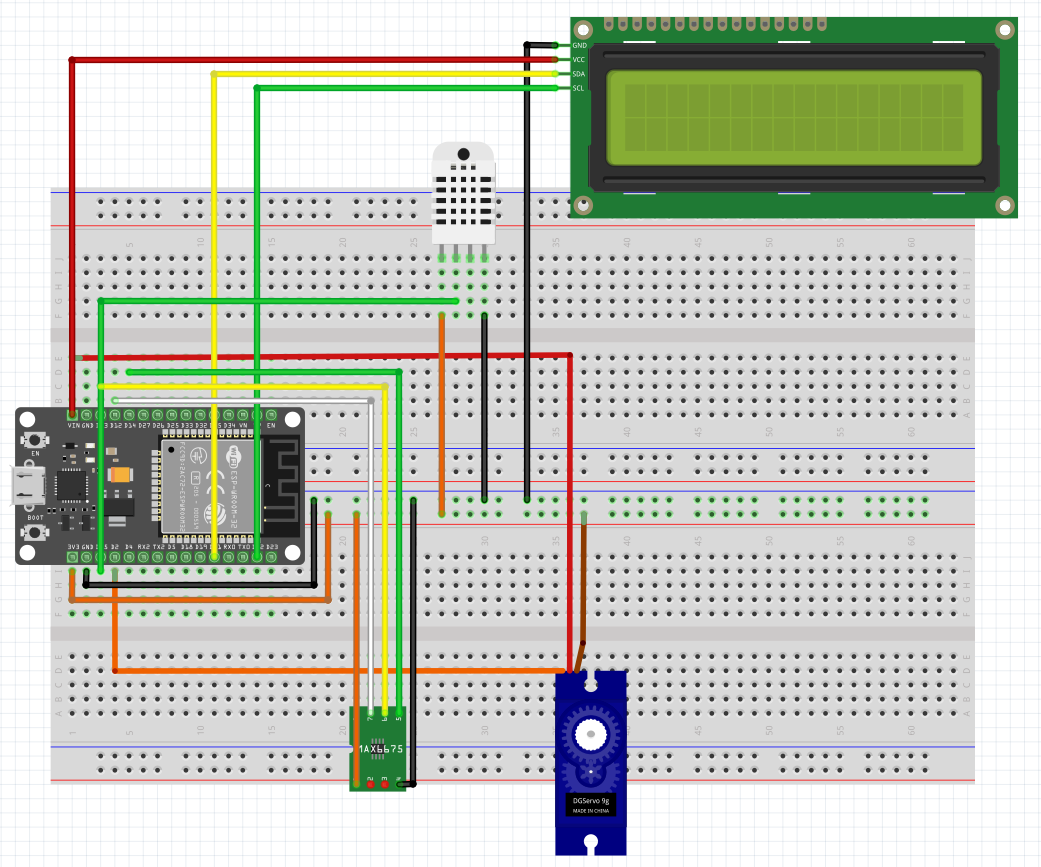
\includegraphics[width=0.8 \textwidth]{fig/fritzing_bredboard_v1.png}
\caption{Wizja elementów sterownika. Opracowanie własne.}
\label{fig:wizja}
\end{figure}
 
 \section{Dalsze kierunki rozwoju}
 W tej części zostaną opisane możliwe kierunki rozwoju sterownika.
 
 Integracja z systemem odzyskiwania ciepła ze spalin.
 \ldots
 

 \chapter{Charakterystyka metod obsługi} 
 Obsługa w pełni manualna - wymaga stałego nadzoru nad przebiegiem spalania. Jest bardzo absorbująca. Łatwo prowadzi do przekroczenia pożądanych temperatur. Pogarsza efektywność procesu spalania co prowadzi do obniżenia sprawności kotła, większego zapotrzebowania na opał, a w konsekwencji znacznie wyższych kosztów ogrzewania.
 
 Obsługa półautomatyczna - pozwala na samodzielną pracę urządzenia pomiędzy momentami dokładania paliwa. Możemy ją podzielić na:
 mechaniczną - głowica termostatyczna połaczona z mechanizmem dźwigni, na ramieniu której znajduje się łańcuszek lub linka. Zaletą jest niski koszt.
 elektroniczną - sterownik pokojowy z serwomechanizmem. Umiarkowany koszt rozwiązania. Szerokie możliwości regulacji. Umożliwia dokonywanie nastaw lokalnie lub zdalnie.
 
 Obsługa automatyczna - kocioł z podajnikiem paliwa pracuje samodzielnie do kilku dni. Najbardziej autonomiczne i jednocześnie najdroższe rozwiązanie.
 
 
 \chapter{Przegląd istniejących rozwiązań}
 Szroka gama rozwiązań przeznaczonych do kotłów na paliwo stałe.
 Niewielka ilość sterowników przeznaczonych dla kominków - tylko z dodatkową przepustnicą co ogranicza możliwość regulacji (powietrze pierwotne i wtórne).
  
 \chapter{Opracowanie koncepcji}
 
 \chapter{Techniczne środki realizacji}
 Może lepiej umieścić przed rozdziałem \label{rozdz.stworzenie}
 
 \chapter{Wybór podzespołów}
 ESP32 - układ SoC, następca ESP8266, wbudowane wi-fi, bluetooth, dwa rdzenie, energooszczędnośc, stosunkowo niska cena, gotowy moduł pozwalający na wygodne prototypowanie, 
 
 \chapter{Wykonanie prototypu na płytce stykowej}
 Pierwsze kroki - podłaczenie mikrokontrolera oraz 2x16 LCD
 
 \chapter{Stworzenie oprogramowania}\label{rozdz.stworzenie}
 
 \section{Utworzenie projektu}
 Do programowania sterownika wykorzystano środowisko programistyczne CLion wraz z ekosystem PlatformIO.
 Projekt został zainicjalizowany w pustym katalogu poleceniem:
 \begin{lstlisting}
pio init --ide clion --board esp32doit-devkit-v1 
 \end{lstlisting}
 
 
 \section{Portal przechwytujący}
 Aby umożliwić łatwą konfigurację połączenia Wi-Fi w sterowniku wykorzystano bibliotekę WiFiManager która pozwala na automatyczne tworzenie sieci wifi i wystawienia portalu przechwytującego dającego możliwość wybrania i połączenia się z docelową siecią. 
 
 Dla zapewnienia bezpieczeństwa dostęp do sieci wifi jest zabezpieczony prostym hasłem podanym w instrukcji obsługi, a także zapisanym na urządzeniu.
 
 
 
 
 
 \chapter{Przetestowanie oprogramowania}
 
 \chapter{Zaprojektowanie płytki drukowanej}
 
 \chapter{Zaprojektowanie obudowy}
 
 \chapter{Zintegrowanie z Mozilla Gateway}
 
 \chapter{Przygotowanie instrukcji obsługi}
 
 \chapter{Efekt końcowy na tle koncepcji}
 Reflekcja na temat tego jak wygląda to co zaplanowałem w stosunko tego co udało się uzyskać.
 
 \chapter*{Podsumowanie}
 \addcontentsline{toc}{chapter}{Podsumowanie}
 Wnioski, jaką drogę przeszliśmy. Rozdział po rozdziale opisujemy co było wyzwaniem.
 
 \chapter*{Dalszy kierunek prac}
 \addcontentsline{toc}{chapter}{Kierunki dalszych prac}
 Jeśli zaczynałbym projekt z moją dzisiejszą wiedzą jak podszedłbym do problemu. Jak dalej rozwijałbym pracę, jakie dalasze temety zostałyby podjęte. 


% \chapter*{Podsumowanie}

% Nasz wybór (patrz: s.~\pageref{sec:wybor}) miał istotne znaczenie.
% O tym, co było następnie, pisaliśmy w podrozdziale \ref{sec:nastepnie}.
% Konsekwencje\,\ldots

 
  \nocite{*}
% \bibliography{library}
% \bibliographystyle{acm}
 
 \inputencoding{utf8}
 \addcontentsline{toc}{chapter}{Książki}
 \printbibliography[title={Książki},type=book]
 \addcontentsline{toc}{chapter}{Artykuły}
 \printbibliography[title={Artykuły},type=article]
 \addcontentsline{toc}{chapter}{Prace dyplomowe}
 \printbibliography[title={Prace dyplomowe}, type=thesis]
 \addcontentsline{toc}{chapter}{Materiały konferencyjne}
 \printbibliography[title={Materiały konferencyjne},type=inproceedings]
 \addcontentsline{toc}{chapter}{Pozostałe źródła}
 \printbibliography[title={Pozostałe źródła}, nottype=article, nottype=book, nottype=inproceedings, nottype=thesis]

 

 \end{document}

